\documentclass[12pt,english]{article}
\usepackage[T1]{fontenc}
\usepackage{mathptmx}
%\renewcommand{\familydefault}{\sfdefault}
\usepackage[latin9]{inputenc}
\usepackage{multirow}
\usepackage{multicol}
\usepackage[letterpaper]{geometry}
\geometry{verbose,tmargin=2cm,bmargin=2cm}
\usepackage{float}
\usepackage{amstext}
\usepackage{amsmath}
\usepackage{mathptmx}
\usepackage{amsthm}
\usepackage{array}
\usepackage[capposition=top]{floatrow}

\newtheorem{hypothesis}{Hypothesis}
\usepackage[title,titletoc]{appendix} 
\usepackage{multirow}
\newtheorem{result}{Result}
%\usepackage{theorem}
\newtheorem{hypo}{Hypothesis}
\usepackage{harvard}
\usepackage{graphicx}
\usepackage{ amssymb }
\usepackage{url}
\usepackage{epstopdf}
\usepackage{caption}
\usepackage{subcaption}
\usepackage{natbib}

\graphicspath{{figures/}}

\usepackage{setspace}
\usepackage{esint}
\doublespacing
\usepackage{babel}
\DeclareMathOperator*{\med}{med}

\hyphenation{parti-cularly}

\begin{document}

\title{Strategic commitment in an experimental conflict game}

\author{Jean Paul Rabanal
\footnote{Department of Banking and Finance, Monash University}  \and Philip Grossman
\thanks{Department of Economics, Monash University.}  \and Youngseok Park\thanks{Department of Economics, Colby College} \and Olga A. Rud \footnote{Department of Economics, University of Melbourne} }\date{\today}
\maketitle
\begin{abstract}
We conduct a laboratory experiment to study the role of strategic commitment in solving the cycle of conflict in the game of Baliga and Sj\"ostr\"om (2004). In the baseline treatment, players simultaneously commit to play either a Hawkish or Dovish action. We add a sequential and an endogenous move treatment, where in the former, the first mover is exogenously selected and in the latter, players self-select the order of play. The two treatments serve to relax the commitment for the second mover. We find that (i) the cycle of conflict is significantly reduced in the last two treatments and (ii) the outcome in the endogenous move treatment is mainly driven by gender. Men are willing to play more often the risky Dovish action compared to women. 
\end{abstract}

\textbf{Keywords:}
strategic complementarity; type uncertainty; endogenous timing; gender; laboratory experiment\\
\textbf{JEL codes:} C72, C92, D82, D91
\newpage
\section{Introduction}
\label{sec:intro}

Recent government attempts to end the arms race, whether domestically in Colombia, or internationally between North and South Korea, are reminiscent of the early insights on strategic commitment by Thomas Schelling in "The Strategy of Conflict," where he suggests that commitment can lead to a Pareto superior outcome. The idea of commitment as a way to improve social welfare has been the motivation for a number of studies in non-cooperative game theory as well as in experimental economics.\footnote{Hamilton and Slutsky (1990), Maliath (1993),  and Normann (2002) study duopoly games; Andreoni (1998) studies public goods;  Dasgupta (2007) and Farrell and Saloner (1985) study coordination games; and Baik and Shogren (1992) study contest games.  In games of complete information, based on Hamilton and Slutsky (1990), experimental work has studied whether Stackelberg leadership will emerge in duopoly games (strategic substitutes) where players set quantities. Evidence (Huck et al. 2001, 2002) shows that Cournot and collusive outcomes appear more often than predicted by theory. In an environment of asymmetric capacities and price-setting, Mago and Dechenaux (2009) shows that the large capacity firm leads with high prices, and the small capacity firm follows. For an overview of the experimental literature on conflict games, please refer to Kimbrough et  al. (2017). }  However, we still lack evidence on how strategic commitment can solve the cycle of conflict. Baliga and Sj\"ostr\"om (2004, hereafter BS04) provide perhaps the best known game theoretical approach to this problem. In the present paper, we expand on the work of BS04 to evaluate the role of commitment on social welfare outcomes using experimental methods.  


In BS04, players simultaneously decide whether to choose an aggressive (hawkish, $H$) or a peaceful (dovish, $D$) action in an environment of incomplete information. That is, each player knows their own payoff to playing $H$, but not that of the counterparty. The payoff for playing $H$ is independently drawn for each player and can be viewed as a representation of player type ---more hawkish or less hawkish. We focus on the strategic complements environment of BS04, where a player has an incentive to play $D$ ($H$) when the counterparty does so as well. The BS04 equilibrium solution suggests that player types at or below a unique cutoff strategy will play $D$.\footnote{In contrast to most global games literature (Carlsson and Van Damme, 1993; Morris and Shin, 2005), BS04 and Farrell and Saloner (1985) assume that types are not correlated and receive no signals about counterparty payoff. }


To test the role of commitment in a strategic complement game, we add two treatments to the original simultaneous move game (CGO): (i) a sequential move game (CGS) and (ii) endogenous order of play (CGE), with action commitment. Our two treatments draw on the theoretical framework of Park and Rabanal (2018). In the CGS environment, order of play is sequential and exogenously determined following commitment to an action ($H$ or $D$). Equilibrium play requires a higher cutoff strategy relative to the simultaneous move game, which means that the dovish action is selected more often in the CGS game. In a CGE game, on the other hand, players simultaneously self-select the order of play, after committing to an action. This can lead to three different scenarios: (i) a simultaneous-move game if both players choose to move first, (ii) a sequential-move game in which players somehow coordinate to move in different periods, and (iii) a simultaneous-move game if both players choose to move second. Therefore, the CGE game can lead to two possible equilibria. One equilibrium resembles the outcome under simultaneous play, while the other has a majority of players committing to $D$, leading to a Pareto superior outcome. 

The experimental results suggest that a sequential move game can improve welfare, though not to the extent predicted under the assumption of risk neutrality. Moreover, we find that in an endogenous order of play, outcomes are separated by gender. In the experiment, we elicit cutoff strategy for each player and find no significant differences in cutoff decisions across gender in the CGS game. Note that the CGE game adds strategic uncertainty to the environment. A player who commits early to $D$ is uncertain not only about the strategy of the counterparty, but also of the environment. That is, will the players play a sequential game or a simultaneous game? Women react to increased uncertainty by adopting a strategy that is similar to the one we find in a CGO environment, choosing a lower cutoff and playing $H$ with higher frequency. Such strategy minimizes risk when a player expects the counterparty to play $H$ with a sufficiently high probability. Men, on the other hand, increase their cutoff strategy, which has statistic and economic significance. The willingness to play $D$ with higher probability, while risky, can lead to a Pareto superior outcome. 

Our study is related to previous literature on cutoff strategy in games of incomplete information with strategic complements.\footnote{For a theoretical description on the role of pre-commitment in games of complete information with strategic complements and/or substitutes, please refer to Eaton (2004).} Brindisi et al. (2014) find that in an investment game with correlated player types (a joint investment opportunity) endogenous timing improves social welfare. Specifically, the results suggest that coordination is higher under endogenous timing, though it is lower than predicted. In the simultaneous move game, subjects use a cutoff strategy that deviates from theory, and approaches payoff dominance which is similar to what we observe in our CGO treatment. Other games of incomplete information (Van Huyck et al., 2018) and complete information (Heinemann et al., 2004 and Duffy and Ochs, 2012) also report similar findings.\footnote{Duffy and Ochs (2012) study the role of endogenous timing in an entry game, and find no difference in behavior relative to the simultaneous move game.} However, for some simultaneous move games of incomplete information risk dominance becomes an important factor in strategy selection (Cabrales et al., 2007).  


According to the experimental results of Heggedal et al. (2018), risk aversion can significantly deter a first mover from committing to an irreversible action. The study tests the main predictions of Farrell and Saloner (1985), which is also closely related to the environment in BS04. In stage one, players simultaneously decide whether to (i) remain at status quo (known payoffs) or (ii) choose an alternative (risky payoff) that is irreversible. In stage two, only those players who have not yet committed choose between the two alternatives. If no player committed in stage one, second stage decisions become simultaneous. The results show that players are willing to commit when the risk of failure is low and that they follow the equilibrium cutoff strategy. When the risk of failure is high, players are less willing to commit and the behavior deviates from the theoretical prediction. These findings are similar to what we observe in our sequential and endogenous treatments. In addition, our results also suggest that men are more willing than women to accept the risk of failure (or success). 

In a survey on gender risk attitude, Niederle (2016) finds that while differences in preferences exist, they vary considerably depending on the elicitation method. Our results appear to support this notion. In the CGO and CGS environments, women seem to approach risk similar to men when selecting the cutoff strategy. However, when the order of play is endogenously determined, as in CGE, gender difference appears. Our experimental design does not reveal to the subjects that the study aims to measure gender differences. Moreover, all sessions have a fairly balanced gender composition within groups. 

Babcock et al. (2017) find that in mixed groups women play $D$  more often than men in a volunteer game where $H$ is the status quo of not volunteering. It is important to note that their environment is characterized by strategic substitutes, while ours has strategic complements. Therefore, in our setting, there is an incentive to follow a strategy. When group size is increased in volunteer games ($\approx 100$ participants), there is no observable difference in behavior across gender (Kop\'{a}nyi-Peuker, 2018).   

Dufwenberg and Gneezy (2005) compare the performance of men and women in a repeated, minimum-effort coordination game with strategic complements. While the gender composition of teams was not announced (single gender), participants could observe other players. The study found no significant difference in chosen effort. Di Girolamo and Drouvelis (2015) analyzed the performance of single gender and mixed gender groups in the same game as Dufwenberg and Gneezy (2005). In the single gender treatments, subjects know the gender of their team members; in the mixed gender treatment, subjects are unable to discern the gender mix of their team. Di Girolamo and Drouvelis found no significant differences in chosen effort across the three treatments. Similarly, in another coordination game with strategic complements,  Heinemann et al. (2009) find no observable difference across gender.\footnote{In a different environment, regarding the effect of gender on leader choices, Grossman et al. (2015) find that women leaders are more willing to take risks in a three-person investment game (strategic substitutes) when playing with other women. The responders, on the other hand, behave similarly regardless of leader's gender.} 
 

%Kiss et al. (2014) study gender differences in bank runs. In this games, the strategic complementary arises from the fact that agents best response is to withdraw if others do so, even though they could obtain higher returns if a sufficient number of participants do not liquidate until maturity.\footnote{There is large tradition of modeling bank runs or attacks using techniques from global games.  For example, see Goldstein and Pauzner (2004, 2005), Morris and Shin (2003, 2004a, 2004b), Guimaraes and Morris (2007), Rochet and Vives (2004), among others.} Kiss et al. do not find significantly differences on withdrawing rates across gender, except when the choices are revealed to other participants. In that case, women decrease their withdrawing rates compared to men. Perhaps, it is worth noticing that BS04 game can easily be understood as a liquidity model. Players are uncertain about the liquidity shock faced by the counterparty and make a decision between withdrawing ($H$) or keeping their funds invested ($D$). Our results then suggest that when players select the order of play and commit to an action, women prefer to withdraw more often than men. 



\section{The conflict game}
\label{sec:model}
We model our environment after the one shot conflict game of BS04. In this game of incomplete information, player $i\in\{A,B\}$ can pursue either a hawkish (aggressive) action ($H$), or a dovish (peaceful) action ($D$). The action space for a player can be specified as $s\in\{H,D\}$, and leads to the following payoff matrix
\begin{equation}
\begin{pmatrix}
x_i & \mu+x_i \\
k-d & k 
\label{t:payoff}
\end{pmatrix}.
\end{equation}
where $k=100$, $\mu=10$ and $d=95$. When both players play $H$, each player receives $x_i$, which is an idiosyncratic private payoff that is independently drawn from a uniform distribution $F\in [0,k]$. Therefore, the idiosyncratic $x_i$ can be thought of as Hawk type, where some players are revealed to be more Hawkish, and reap more benefit from action $H$, and some are revealed to be less Hawkish and see a lower return to playing $H$. If both players choose the peaceful action $D$, then the payoff to each player is a constant $k$. If player $i$ plays $D$, while player $j\neq i$ plays $H$, then the payoff to player $i$ is $k-d>0$, where $d$ can be considered a cost of a peaceful action when the opponent is aggressive. On the other hand, if player $i$ plays $H$ and player $j\neq i$ plays $D$, then the payoff to player $i$ is $\mu+x_i$, where $\mu (<d)>0$ can be viewed as a marginal benefit of an aggressive action when the opponent is peaceful. 

The Bayesian Nash Equilibrium (BNE) can be characterized as a cutoff strategy, following BS04, such that a player with a payout lower than $x_i\leq\hat{x}_{_{CGO}}$ will play $D$, and $H$ otherwise.  When a player is indifferent between $H$ and $D$, we can find the cutoff as the unique fixed point where 
\begin{equation}
\hat{x}_{_{CGO}}= k-d + (d-\mu) F(\hat{x}_{_{CGO}}). \label{eq:cgo}
\end{equation}

\noindent Given that $F(\cdot)$ follows a uniform distribution in the space $[0,k]$, the cutoff point can be rewritten as 
\begin{equation}
\hat{x}_{_{CGO}}= \frac{k\cdot (k-d)}{k-d+\mu}=33. \label{eq:cgosol}
\end{equation}
A possible mechanism for improving welfare in a CGO game is for players to move sequentially (Park and Rabanal, 2018). The order of play can be either exogenously (CGS) or endogenously (CGE) determined. In the former, the order of play is randomly determined while in the latter players self-select the order of play. Social welfare under a CGS game is significantly higher relative to a CGO game. In a GGE game, social welfare may be similar to either the CGO or a CGS environment. That is, the CGE game can lead to multiple scenarios, which we discuss in greater detail further below. We begin by describing the optimal strategy in a CGS game, where a player is randomly selected to move first. 

The cutoff strategy for the first mover in a CGS game shifts to the right of the optimal strategy in a CGO game, such that $\hat{x}_{_{CGO}}\leq\hat{x}_{_{CGS}}$. That is, in order to play $H$, a player in a CGS environment has to be more hawkish, or requires a higher payoff to $H$. The intuition for the rightward shift in the cutoff strategy is fairly straightforward. Consider a first-mover at the original cutoff $\hat{x}_{_{CGO}}$. If the first-mover selects $D$, then she will obtain greater expected profits because the probability that the second mover will play $D$ as well is higher due to strategic complementarity. In other words, the probability that the other players plays $D$ increases from $Pr(x\leq\hat{x}_{_{CGO}}) \equiv F(\hat{x}_{_{CGO}}) $ in the CGO game to  $Pr(\mu+x_j\leq k) \equiv F(k-\mu)  $ in the CGS game. The unique Perfect Bayesian Nash Equilibrium (PBNE) where the first mover uses the cutoff strategy can then be defined as
\begin{equation}
\sigma_i(x_i)=D \quad \text{if} \ \ x_i\leq \hat{x}_{_{CGS}} \equiv k-\mu=90. 
\end{equation}

\noindent \textit{Proof:} If the first player $i$ plays $H$, then the second player will play $\sigma_j= H$ if $x_j> k-d$ and $\sigma_j= D$ otherwise. Similarly, if the first player plays $D$, then the second player will play $\sigma_j= H$ if $\mu+x_j> k$ and  $\sigma_j= D$ otherwise. Given the best response strategy of the second player, the first is indifferent between $H$ and $D$ when the payoffs of $H$ and $D$ are equal, or $x_i + \mu F(k-d) = k - d(1-F(k-\mu))$ or $x_i=\hat{x}_{_{CGS}}\equiv k-\mu$ $\blacksquare$

Next, we discuss the CGE game where the players self-select the order of play. The timing of the game proceeds as follows:

\textit{Stage 0:} Each player $i$ selects a cutoff strategy, indicating a set of values where $\sigma_i(x_i)=H$, and then observes own type $x_i$, but not the other player's type $x_j$ where $j\neq i$.

 \textit{Stage 1:} Both players simultaneously decide the period they will play the game $t=1,2$. 

\textit{Stage 2:} The conflict game is played by the move structure determined in Stage 1. The commitment to the cutoff strategy is not binding for the player $i$ if and only if $t_i=2$ and $t_j=1$. 

The CGE game predictions follow the CGO and CGS solutions. Note that if both players commit to play at $t=1$, then the environment is similar to a simultaneous move game, where the equilibrium follows the cutoff strategy specified in BS04. Therefore, in one possible equilibrium, $\hat{x}_{_{CGE}}=\hat{x}_{_{CGO}}=33$ and
no player has incentive to deviate. Alternatively, players can coordinate and follow the order described in the CGS game, which leads to another equilibrium where type $x\leq \hat{x}_{_{CGS}}\equiv 90$ will select $t=1$ and commit to $D$, while type $x>\hat{x}_{_{CGS}}$ will wait to play at $t=2$. Again, under this equilibrium, players do not have incentive to deviate. 

\noindent \textit{Proof:} See Park and Rabanal (2018) $\blacksquare$

We summarize all theoretical predictions that will be tested in the laboratory as follows,

\noindent \textbf{Prediction 1}
\textit{In the simultaneous conflict game  subjects play at or above the cutoff strategy $\hat{x}_{_{CGO}}=33$.}

We reconcile the theoretical solution in CGO to experimental evidence when forming our first prediction. In the laboratory, human subjects play $D$ more often than suggested by the NE prediction. For example, Evdokimov and Garfagnini (2018) find that in the simultaneous move game subjects play $D$ at a rate of 64 percent compared to 50 percent predicted by the NE of the conflict game.\footnote{Evdokimov and Garfagnini (2018) work with slightly different parameter values compared to ours. In their experiment, they use $k=95$, $\mu=10$ and $d=85$. The main purpose of their study is to test the predictions of Baliga and Sj\"ostr\"om (2012) where a third-party can manipulate the two-player conflict game. They find that third-party communication is not strategic. Our experiment does not include a third-party. However, theoretically, the sequential game outcomes presented in this paper is robust to the presence of such third-party.} 

\noindent \textbf{Prediction 2}
\textit{In the sequential CGS game, the first mover will increase the cutoff strategy compared to the cutoff in CGO game. }

Note that the equilibrium predictions in CGS and CGO games of 90 and 33 respectively are far apart. This allow us to observe meaningful differences when players chose cutoff values greater than NE prediction as described in Prediction 1. In terms of payoff difference, the gain in expected payoff is equal $d\times \left( F(\hat{x}_{_{CGS}})-F(\hat{x}_{_{CGO}}) \right)=95\times( 90-33)/100=50$ points or 137 percent relative to the payoff in CGO game predicted under the NE. 


\noindent \textbf{Prediction 3a}
\textit{In the endogenous CGE game a player will behave as the
  CGO game. }


\noindent \textbf{Prediction 3b}
\textit{In the endogenous CGE game a player will behave as the CGS game.}

Up to this point, we are uncertain about the type of equilibrium that would prevail in our experiment. Our two different Predictions 3a and 3b reflect our priors. 


\noindent \textbf{Prediction 4}
\textit{The probability of observing a $DD$ outcome is greater or equal in the CGS and CGE games compared to the simultaneous game CGO.}

It is quite evident that coordination to the $DD$ outcome should be higher in the CGS game compared to the simultaneous game. The worst outcome in the CGE game is the one predicted for CGO game while the CGS game provides an upper bound given that eliminates any possible coordination issues between the players that simultaneously opt for the order of play. Henceforth, we expect that frequency of $DD$ under the CGE game is at least as the one observed in the CGO game. 

\noindent \textbf{Prediction 5}
\textit{There is not any gender difference in playing H across the
  three games.}

Even though Babcock et al. (2017) find that women are more accommodating in playing $D$ than men, risk aversion deters subjects to commit and improve social welfare (see  Heggedal et al., 2018). We do not take any strong position on risk attitudes across gender following Niederle (2016) overview of the literature. 


\section{Laboratory procedures}
\label{sec:game}

The experiment was conducted at the Rosario Experimental and Behavioral Economics Lab (REBEL) of the Universidad del Rosario, Colombia. Participants included undergraduate students from all fields and were recruited online via ORSEE (Greiner, 2015). Subjects were part of one of the three treatments (between design) ---CGO, CGS and CGE---  with each treatment consisting of 5 practice periods and 11 paid periods.\footnote{For the documentation in Spanish, language used in the sessions in Colombia, please contact the corresponding author.} In total, we conducted nine sessions, with two silos per session. In each silo, a treatment included 12 subjects with gender balance participation. Each participant meets another participant once and only once (perfect stranger matching).\footnote{Alternatively, one can employ a mean matching protocol as in Hawk-Dove population games (Oprea, et al., 2011 and Benndorf, et al. 2016) for the simultaneous move game. A mean matching in the endogenous timing game brings technical difficulties in its implementation.}  The participants were not informed that the study also focuses on analyzing possible gender differences.

\begin{center}
\begin{figure}[ht]
\centering{}%
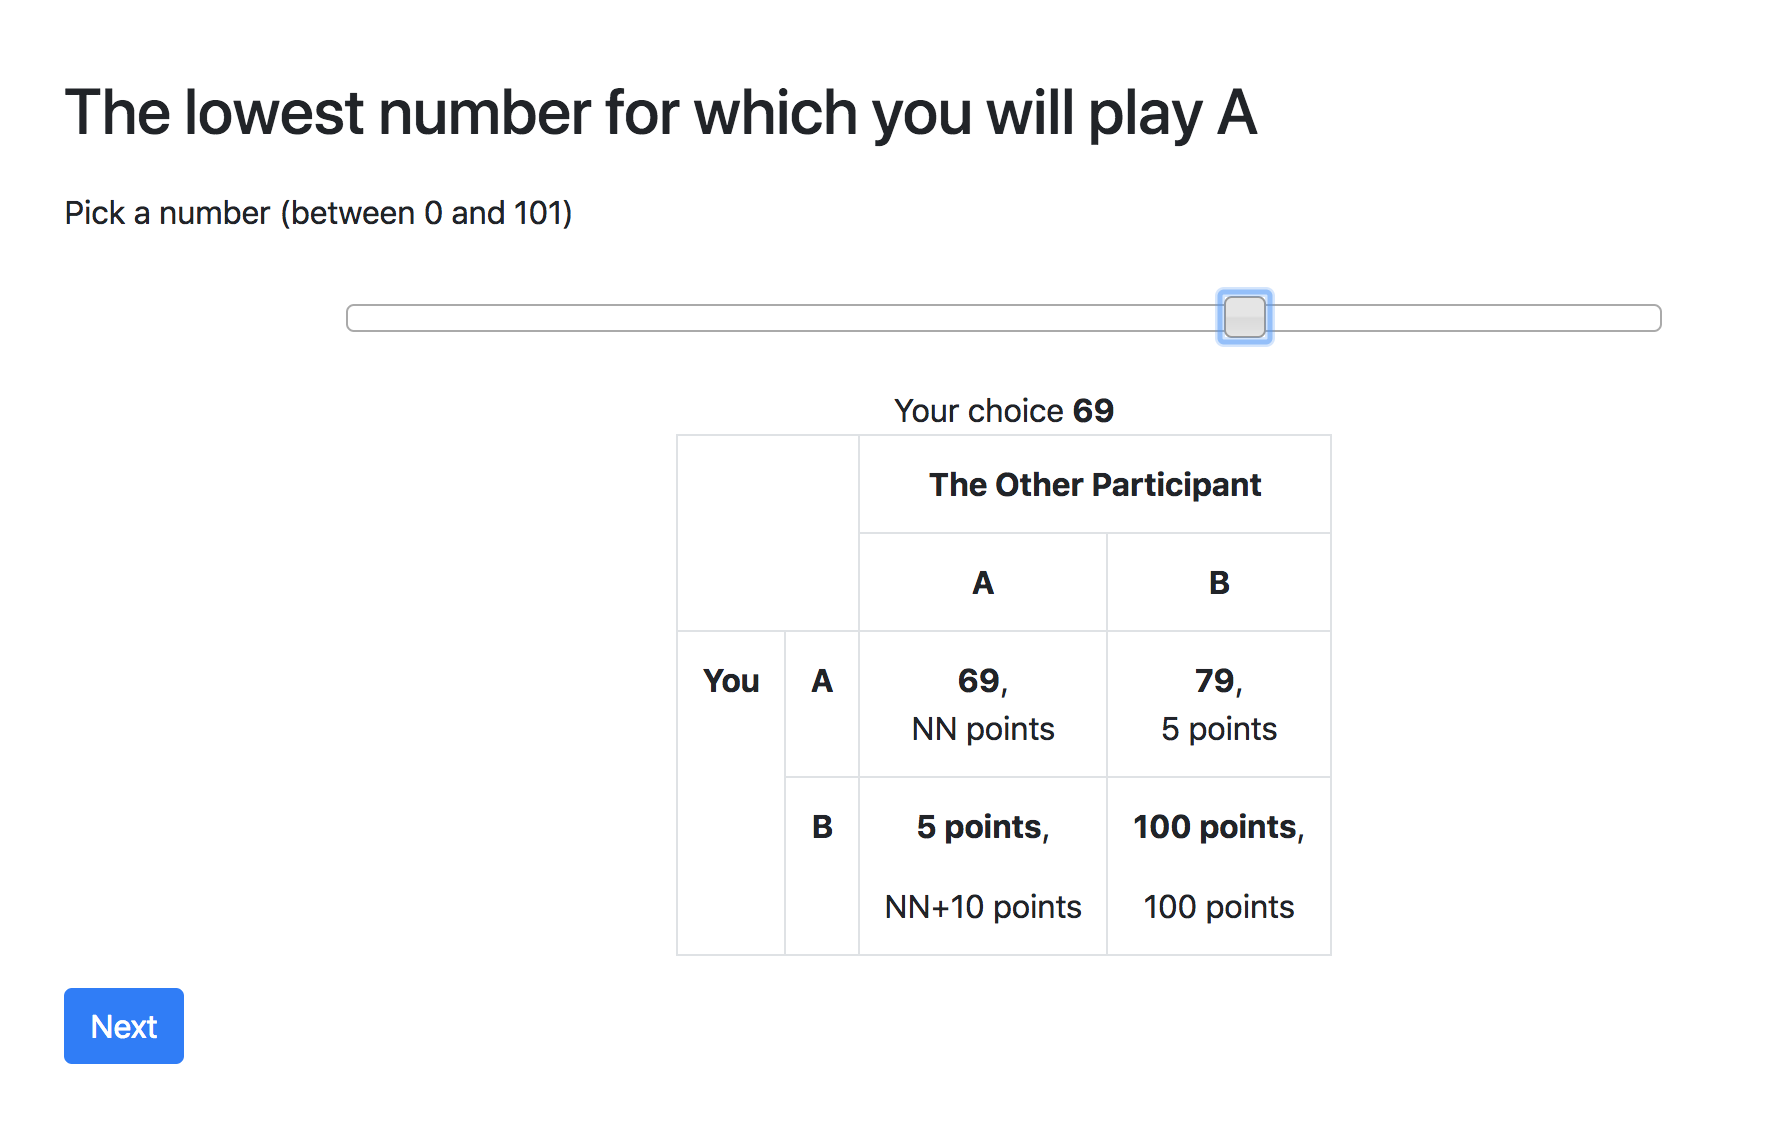
\includegraphics[scale=0.4]{cutoffen.png}%
\caption{User-Interface cutoff decision} 
\label{fig:ui}
\end{figure}
\end{center}

In each silo, the game started with five solo practice rounds. The counterparty is a robot that plays the NE prediction. The subject's task is to pick the minimum number of $x$ in the interval $[0,101]$ for which she will play $H$ (labelled $A$ in the experiment). That is, we directly ask the subject to select a cutoff strategy without having knowledge of her value of $x$ as well as the counterparty's value.\footnote{A similar cutoff elicitation task, but without our slider, also appears in Duffy and Ochs (2012). They find that the elicited cutoff is consistent with the actual binary choices in their entry game. Additionally, Van Huyck et al. (2018) survey their participant about how they play the game. 72 percent of their participants reported that they were using a threshold. Similar to the behavior observed in our experiment, Duffy and Ochs also find that there is a significant variation of cutoff strategies across subjects. } The user-interface designed in oTree (Chen, et al., 2016) is depicted in Figure \ref{fig:ui}. Specifically, in order to select a cutoff value, the participant uses the mouse to move the slider. Then, to confirm her choice, the participant clicks on the button ``Next." Thus, a subject who wants to play always $D$ ($H$)  moves the slider to the extreme right (left). The user-interface also presents the updated payoff matrix with the cutoff selection. In the payoff matrix, the unknown value of $x$ for the counterparty is depicted as $NN$.

Following the five practice rounds, subjects in all treatment make the cutoff choice simultaneously. Recall that the subject does not know the counterparty's gender. The next steps after choosing the cutoff value vary according to treatment. We summarize the different steps in Table \ref{table:time}. 

\begin{table}[ht]
\begin{center}
\begin{tabular}{l|m{2.4cm}|m{3.5cm}|m{4cm}}
  Step & CGO & CGS & CGE\\
  \hline 
I & cutoff & cutoff & cutoff \\
\hline
II& $x_i$ is revealed; H if $\mtext{cutoff}\leq x_i$ & $x_i$ is revealed; H if $\mtext{cutoff}\leq x_i$ for 1st mover (randomly chosen)
& $x_i$ is revealed; choose $t=\{1,2\}$ with action commitment defined according to $\mtext{cutoff}$\\
\hline
III & - & 2nd mover picks \textbf{s} & 2nd mover ($t=2$) picks \textbf{s} if other chose $t=1$. Otherwise, the game is a oneshot.

\end{tabular}
\end{center}
\caption{Timeline for each treatment}
\label{table:time}
\end{table}

In the CGO game, the value of $x_i$ is revealed to player $i$. The subject plays $H$ if her cutoff choice is smaller or equal than $x_i$. She plays $D$ otherwise. Given the actions $H$ or $D$ for both players, payoffs are computed according to the payoff matrix in equation (\ref{t:payoff}). 

In the CGS game, a first-mover is selected randomly after all subjects completed the cutoff choice. This procedure helps us to collect cutoff information for all subjects independently if they are first or second movers, and allow us to have a balance number of silos across treatments. Here, it is also important to emphasize that all subjects know that their cutoff decisions are binding (relaxed) if they are first (second) movers. The second mover picks an action $s\in\{H,D\}$ conditional on the first-mover's action. That is, the second mover does not face the same payoff matrix presented to the subjects in the CGO game. Instead, the payoff matrix in the CGS game only shows the action selected by the first mover. 

In the endogenous timing game (CGE), subjects commit to the action mapped from the cutoff choice. They now decide when to play the game. If both players select the same period of play, then the game becomes a one-shot game. If one player picks the first period while the other player picks the second period, then we are in the CGS game, where the cutoff choice for the second mover is relaxed. The second mover makes a decision knowing what the first mover played. 

At the end of each round for all treatments, we provide feedback regarding the participant and the counterparty choices as well as payoff information. After the 11 rounds were completed, the total points were converted to COL at the exchange rate of COL 20 per point and paid in cash in addition to the show-up fee of COL 10,000 (\$ 3.3). Table \ref{session} presents the average profit as well as other relevant information per treatment. 

\begin{table}[ht]
\centering
\begin{tabular}{lcccc}
  Treatment & Groups & Subjects per group & \% of women & Profit (points)\\
  \hline
  CGO & 6 & 12 & 51 & 63.8 \\
  CGS & 6 & 12 & 51 & 77.8 \\
  CGE & 6 & 12 & 47 & 74.6 \\
\hline
Total & 18 & 216 &  50 (mean) & 72.1 (mean)\\
\end{tabular}
\caption{Sessions overview }
\label{session}
\end{table}


\section{Results}
\label{sec:results}

We start presenting the pooled data across all treatments in Figure \ref{fig:cutpooled}.\footnote{The data collected from the experimental sesssion as well as the data analysis included in this paper can be found at \url{https://github.com/rabsjp/hdseq}.} The mean cutoff is around 50 percent in the CGO game. This behavior is consistent according to previous experimental work (e.g. see Evdokimov and Garfagnini, 2018). We also count the number of outcomes for each cell $HH$, $HD (=DH)$ and $DD$. The $DD$ outcome appears around 30 percent in the CGO game. The off-diagonal cells appear most often (around 50 percent). Both CGS and CGE outcomes are quite different compared to CGO. Subjects in the CGS game increase the mean cutoff value to around 60 percent, and men seem to increase it a bit more compared to women. The sequential move ordering helps achieving coordination to $DD$ or $HH$ outcome, which now appears around 50 percent and 40 percent, respectively. The CGE game presents a similar level of $DD$ outcome compared to CGS, however, the mean cutoff across gender is quite different. Women chose a cutoff similar to CGO game, while men are willing to increase the cutoff, even at a higher rate than in the CGS game. 
\begin{center}
\begin{figure}[ht]
\centering{}%
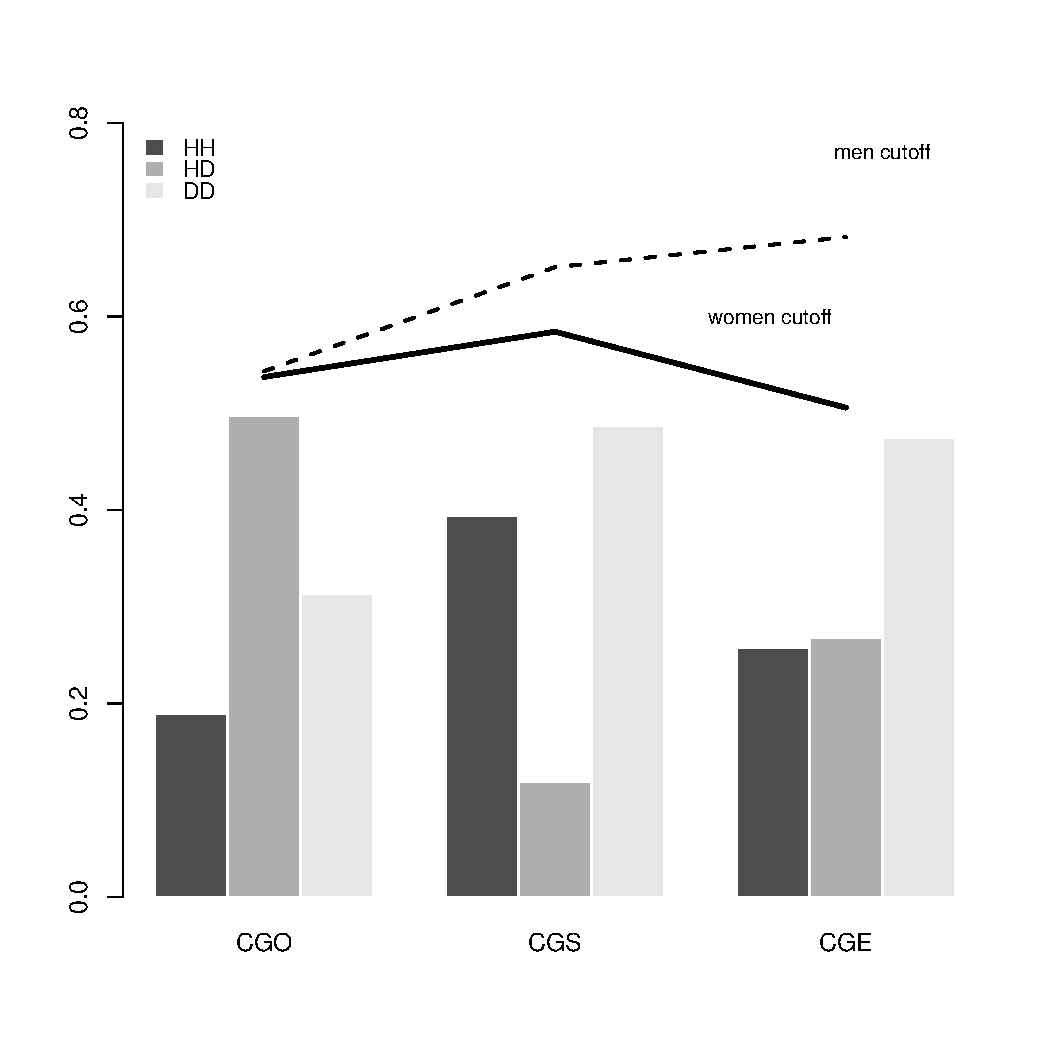
\includegraphics[scale=0.5]{jointcut.pdf}%
\caption{Cutoff strategy and cell relative frequencies across treatments (pooled data)} 
\label{fig:cutpooled}
\end{figure}
\par\end{center}

We further analyze the gender differences in the CGE game according to the play and move ordering. Figure \ref{fig:cgepooled} presents in the first two columns the move ordering across gender. It is quite evident that men prefer to move second while women choices are fairly distributed across both periods. We observe that men play $D$ more often than women in both periods, which is consistent with the different cutoff strategies illustrated in Figure \ref{fig:cutpooled}.
\begin{center}
\begin{figure}[ht]
\centering{}%
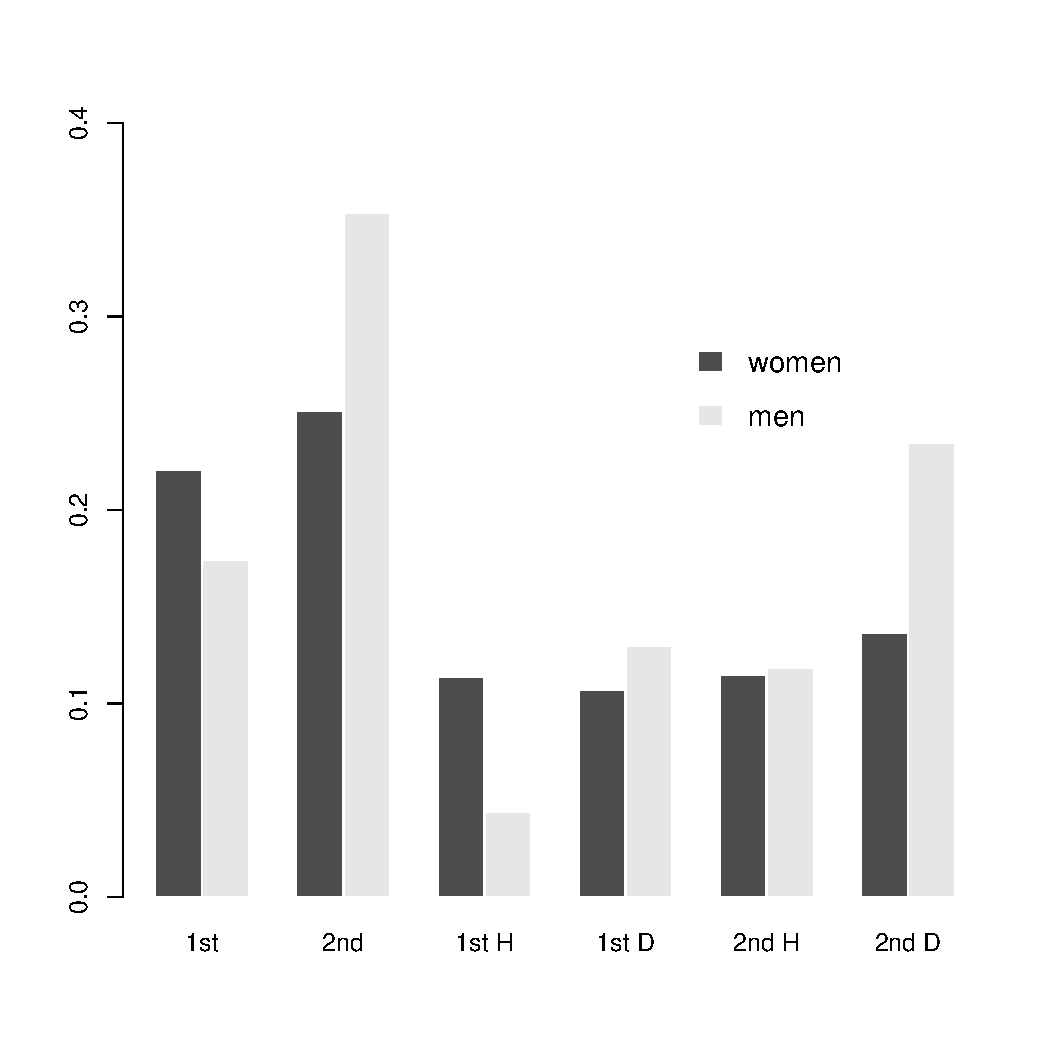
\includegraphics[scale=0.5]{countgendermoveplay.pdf}%
\caption{Play and move ordering in CGE game} 
\label{fig:cgepooled}
\end{figure}
\end{center}
Regarding the type of encounter observed in CGE, Table \ref{tab(CGE)} presents the frequency of the cells $HH$, $HD(\equiv DH)$ and $DD$ tabulated according to the type of encounter, i.e. one-shot in the first period, one-shot in the second period and a sequential order. About 52 percent of encounters occur in a sequential order. Of those, 56 percent lead to the $DD$ outcome. Most of the simultaneous encounters happen in the second period, and 41 percent of them lead to $DD$.  

\begin{table}[!t]
\centering
\begin{tabular}{lccc}

 & One-shot 1st period & One-shot 2nd period  & Sequential\\
  \hline
  $HH$ &  2.27 & 5.56 & 17.93 \\
  $HD$ & 5.81 & 15.91 & 5.05 \\
  $DD$& 5.30 & 12.88 & 29.29 \\
  \hline
Total & 13.38 & 31.35 & 52.27\\
\end{tabular}
\caption{Frequency (percentage) of cell played and type of encounter in CGE game }

\label{tab(CGE)}
\end{table}

\noindent \textbf{Result 1}
\textit{The median cutoff strategy in the simultaneous conflict game is 50 percent.}

We take a conservative approach to test our predictions. We compute the median cutoff chosen by a subject throughout rounds 6-11. Figure  \ref{fig:allcutoff} shows the empirical CDF. The median value is 50 percent, and the distribution is fairly uniform with some qualifications. About 20 percent of subjects pick the highest cutoff which means that they are strongly willing to play $D$. Furthermore, there is no significant mass centered around the NE of 33 percent. In fact, the p-value Kolmogorov-Smirnov test strongly rejects that cutoffs in the CGO game are equal or below the NE prediction. 

\begin{center}
\begin{figure}[ht]
\centering{}%
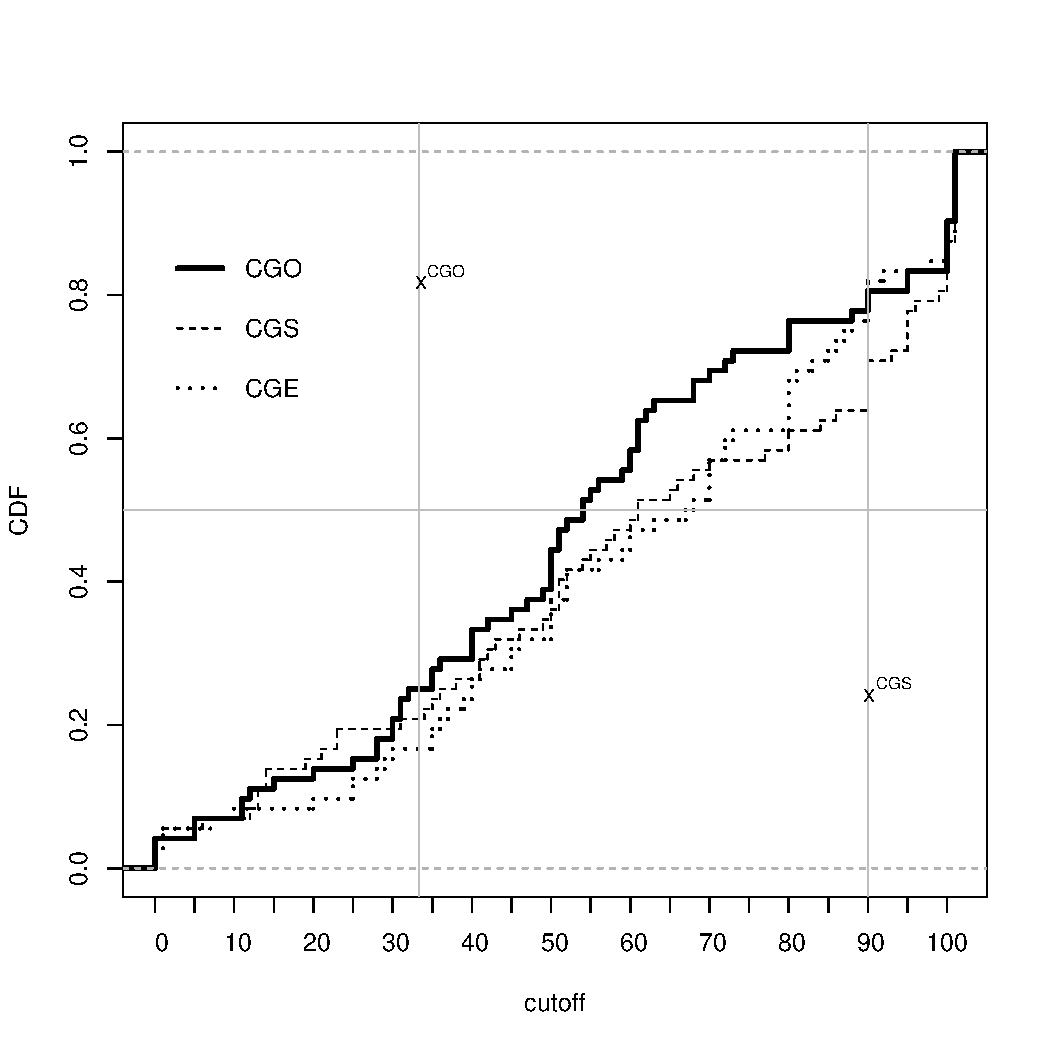
\includegraphics[scale=0.6]{cdfcutoff.pdf}%
\caption{Empirical CDF of cutoff strategies (subject data)} 
\label{fig:allcutoff}
\floatfoot{\footnotesize{\textit{Note: $x^{CGO}$ ($x^{CGS}$) is the predicted cutoff in the CGO (CGS) game.}}}

\end{figure}
\par\end{center}

\noindent \textbf{Result 2}
\textit{In the sequential CGS game, players increase the median cutoff to 66 percent.}

The empirical CDF for the CGS game first order stochastically dominates the empirical CDF for CGO.\footnote{The p-value of a two sided test in which the null is that CGO is larger or equal to CGS is 0.006.} The mass tends to approach the predicted NE of 90 percent, however, still falls short. The median cutoff value is 66 percent. Consistent with the CDF observed in CGO game, we also observe that some players pick either extremely high or extremely low cutoff values. Overall, the majority of players in the CGS game opts for a higher threshold compared to CGO game improving the social welfare. 

\noindent \textbf{Result 3}
\textit{In the endogenous timing CGE game with action commitment, the median cutoff strategy is 70 percent.}

While roughly 25 percent of players select a low cutoff strategy similar to CGO game, the majority of players selects a cutoff value larger than the one observed in the simultaneous game. There is also an important mass (35 percent) selecting values above the predicted NE in the CGS game. The distribution of cutoffs in the CGE game is quite similar to the CGS game. We fail to reject the hypothesis that both cutoffs come from the same distribution.

\noindent \textbf{Result 4}
\textit{The peaceful outcome $DD$ appears more often in CGS and CGE compared to CGO game.}

We compute the frequency in which $DD$ appears in each of the sessions. Table \ref{table:dd} presents the sorted data and the mean per treatment. It is quite evident that $DD$ appears less often in the CGO compared to the CGS and CGE games. Specifically, CGS and CGE do not exhibit the low frequencies of DD ($<0.30$) that appear quite often in the CGO treatment. More formally, nonparametric tests reject the hypothesis that CGO is greater or equal to either CGS (KS p-value of 0.069 and Wilcoxon p-value of 0.018) or CGE (KS p-value of 0.069 and Wilcoxon p-value of 0.015). Additionally, we fail to reject the hypothesis that CGS and CGE come from the same distribution. 

\begin{table}[!t]
\centering
\begin{tabular}{lccccccc}

Treatment & Session 1 & S2  & S3 & S4 & S5 & S6 & Mean\\
  \hline
  CGO &  19.44 & 19.44&  27.78 & 27.78 & 36.11 & 52.78 & 30.56 \\
  CGS & 30.56 & 47.22&  50.00 & 52.78 & 55.56 & 61.11 & 49.53\\
  GGE & 33.44 & 38.49 & 44.44 & 58.55 & 63.89 & 69.44 & 51.39 \\
  \hline

\end{tabular}
\caption{Frequency (percentage) of cell DD played in sessions }
\label{table:dd}
\end{table}

\noindent \textbf{Result 5}
\textit{Gender differences appear in CGE. Men significantly increase the cutoff value, improving the frequency of $D$ relative to women.}

We analyze the cutoffs across gender. Similar to other simultaneous Hawk-Dove games we do not find gender differences in the CGO game. Important differences emerge under endogenous timing. Figure \ref{fig:cdfgender1} presents the empirical CDF cutoff for men and women in CGO (left panel) and CGS (right panel). There are minor differences in the CGO cutoffs, which are not statistically different (KS and Wilcoxon tests). For the CGS game, we observe that for the upper levels of cutoffs, men are willing to pick a high value, surpassing the predicted NE. For cutoff values lower than 60 percent, which correspond to roughly half of the sample, we observe similar behavior across gender. Overall, we fail to reject the hypothesis that men and women cutoff distributions are equal.  

\begin{center}
\begin{figure}[ht]
\centering{}%
\begin{minipage}[t]{0.45\columnwidth}%
\subfloat{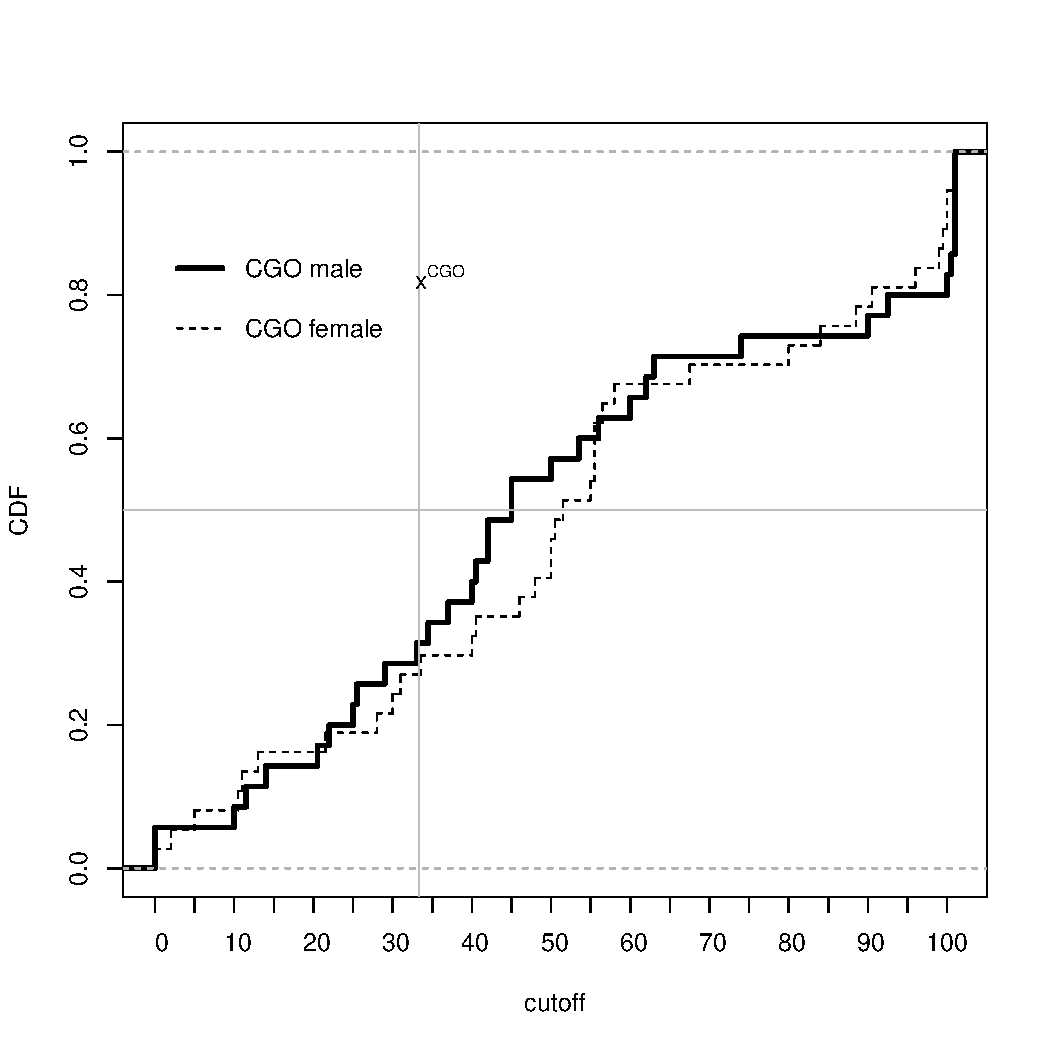
\includegraphics[scale=0.4]{cdfcutoffgender_o.pdf}}%
\end{minipage}%
\begin{minipage}[t]{0.45\columnwidth}%
\subfloat{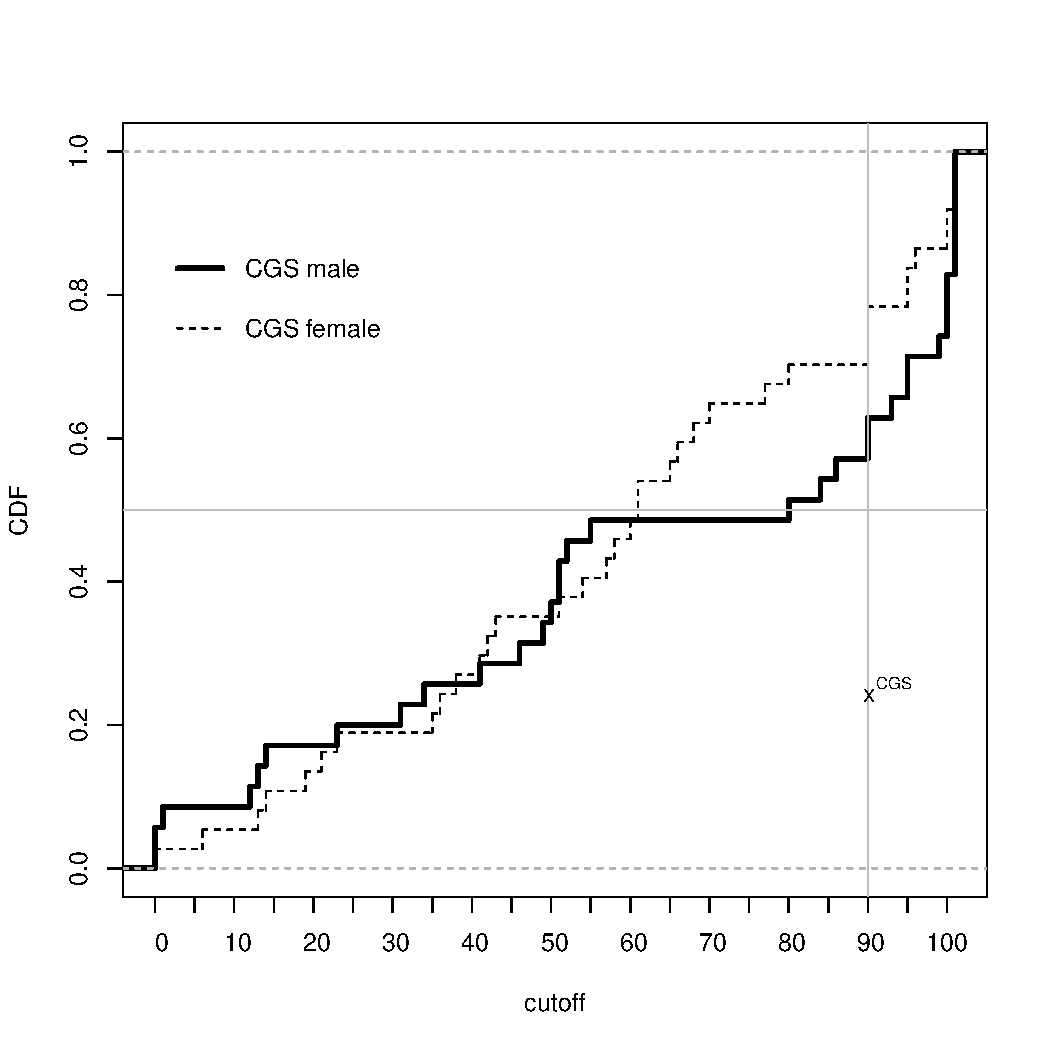
\includegraphics[scale=0.4]{cdfcutoffgender_s.pdf}}%
\end{minipage} 
%\captionsetup{font=large}
\caption{Empirical cutoff CDFs in CGO (left) and CGS (right) games across gender}
\floatfoot{\footnotesize{\textit{Note: $x^{CGO}$ ($x^{CGS}$) is the predicted cutoff in the CGO (CGS) game.}}}
\label{fig:cdfgender1}\end{figure}
\par\end{center}

The significant gender differences appear in the CGE game. The men cutoff choices first order stochastically dominate the women choices as depicted in the left panel of Figure \ref{fig:cdfgender2}. The p-value of a one-sided test in which the null is that men cutoff is equal or smaller than women cutoff is 0.02 for Wilcoxon and 0.01 for KS. The women cutoff distribution resembles the one observed in CGO game. On the other hand, men significantly shift the cutoff to a median value closer to the one observed in the CGS game. In particular, the mass around the high levels of cutoff in both CGS and CGE for men is quite important. About 40 percent of men pick a cutoff value above 90 percent under both CGS and CGE, which is quite different than the behavior observed in CGO. 

The high cutoff value chosen for men translates into a higher frequency of $D$ as shown in the right panel of Figure \ref{fig:cdfgender2}. Corroborating our conclusion achieved after analyzing the cutoff decision, the frequency of $D$ across gender does not show statistically and economically differences in the CGO game or in the CGS game. The difference of play stands out in the CGE with action commitment. Specifically, the results show that men play $D$ at a rate 21 percentage points higher than women. 

\begin{center}
\begin{figure}[ht]
\centering{}%
\begin{minipage}[t]{0.45\columnwidth}%
\subfloat{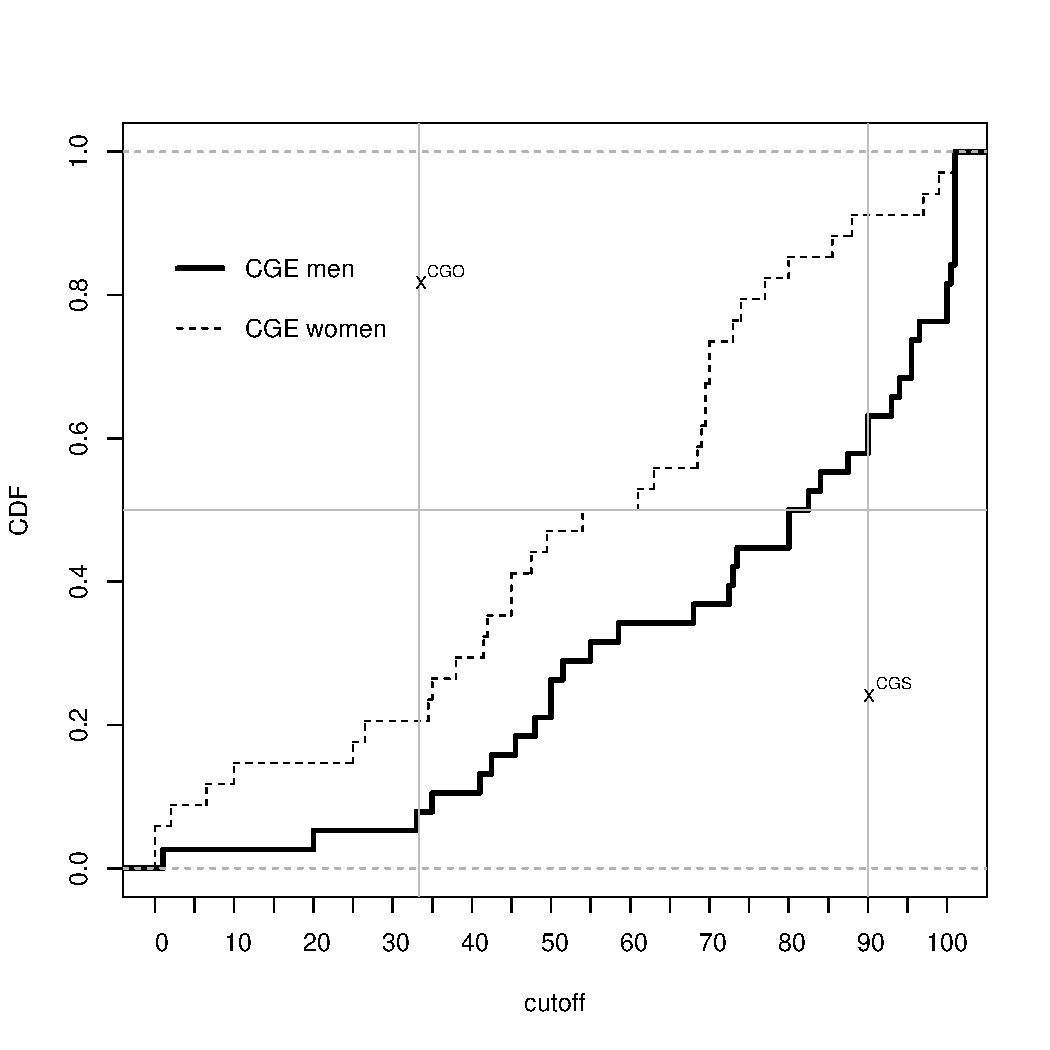
\includegraphics[scale=0.4]{cdfcutoffgender_e1.pdf}}%
\end{minipage}%
\begin{minipage}[t]{0.45\columnwidth}%
\subfloat{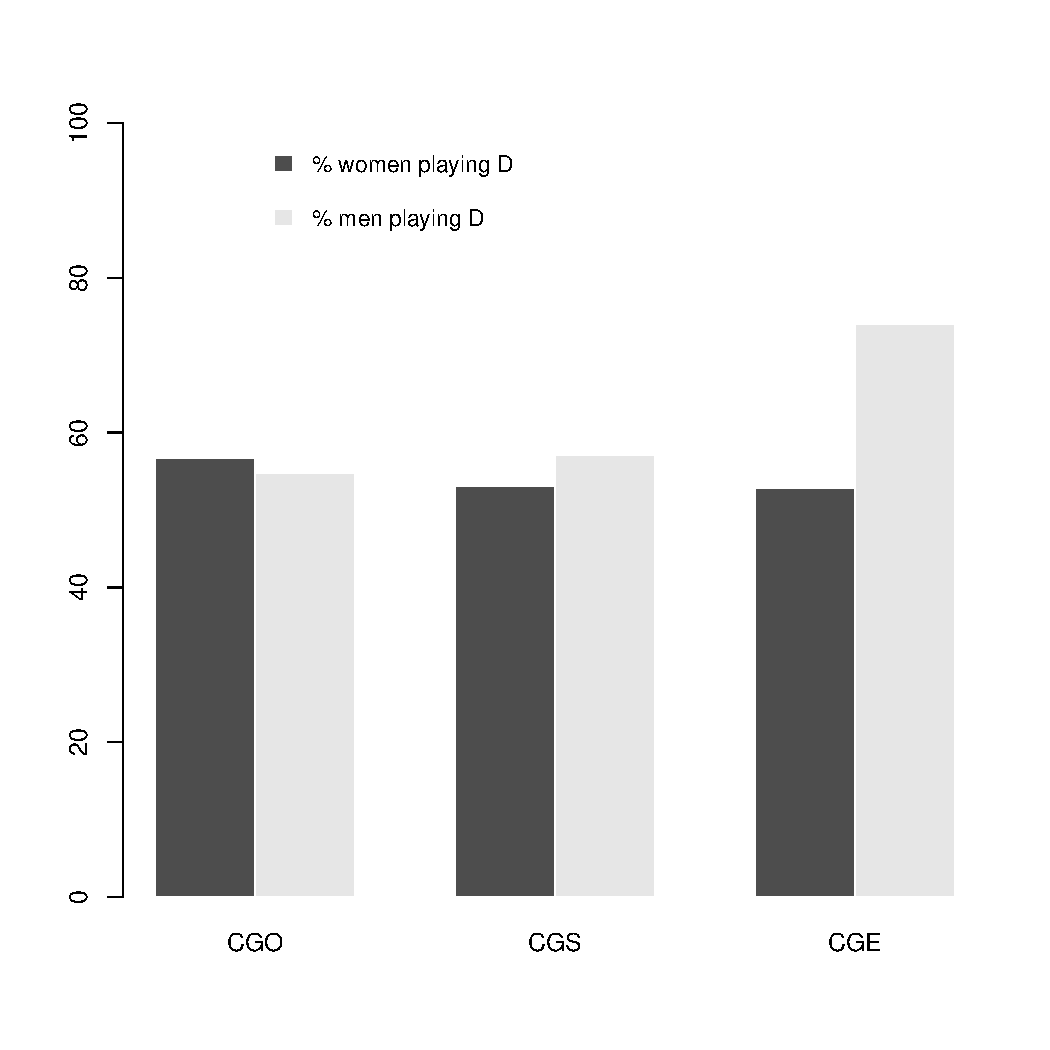
\includegraphics[scale=0.4]{genderplay1.pdf}}%
\end{minipage} 
%\captionsetup{font=large}
\caption{Empirical CDF cutoff in CGE (left panel) and D play (right panel) across gender}
\floatfoot{\footnotesize{\textit{Note: $x^{CGO}$ ($x^{CGS}$) is the predicted cutoff in the CGO (CGS) game.}}}
\label{fig:cdfgender2}\end{figure}
\par\end{center}

\section{Discussion}
\label{sec:discuss}

In this paper, we provide novel evidence regarding gender differences in a conflict game in which players endogenously select the time of play and can commit to either a hawkish or a dovish action. The early commitment to a dovish action is risky because a player can lose 95 percent of the (Pareto) payout when the counterparty plays the hawish action. On the other hand, committing early to a hawkish action leads to a payout of $x$ or $x+10$. The private gain appears when the counterparty plays the dovish action. The experimental results show that men are willing to play more often the risky dovish action compared to women. The gender differences are quite remarkable compared to other environments that remove the strategic uncertainty about the order of player, e.g. a exogenous sequential game and a simultaneous move game. 

The conflict game we study have different applications. It can be interpreted as a bank run model or a game that analyses the imposition of sanctions or tariffs. Here, we elaborate on the first example. In the bank run game, agents withdraw ($H$) or not ($D$) and are uncertain about the liquidity costs of the counterparty. To the best of our knowledge, Kiss et al. (2014) is the only bank run experiment that studies gender differences.\footnote{In the theory side, there is large tradition of modeling bank runs or attacks using techniques from global games. For example, see Goldstein and Pauzner (2004, 2005), Morris and Shin (2003, 2004a, 2004b), Guimaraes and Morris (2007), Rochet and Vives (2004), among others.} Kiss et al. do not find significantly differences on withdrawing rates across gender, except when the choices are revealed to other participants. In that case, women decrease their withdrawing rates compared to men. Thus, Kiss et al. confirm Babcock et al. (2017) results regarding the role of women on helping achieve the social welfare optimum. When subjects face a risky commitment choice, our results show that withdrawing rates are rather higher for women than for men. 

Considering the different conclusions achieved by the literature regarding gender differences in risk attitudes as well as the effect of social norms or culture shaping the gender differences, future field or experimental work can complement the findings documented in the present paper. 
\section{Acknowledgements}
We are grateful for the comments received from Dann Arce, Diego Aycinena, Tim Cason, John Duffy, Dan Friedman, Tom Wilkening and seminar participants at University of Melbourne. This research was supported by funds granted by Colby College. This project was approved by the IRB at Colby College and Universidad del Rosario.

\section*{Appendix A}
\subsection*{Instructions CGE}

Welcome! This is a two player game. Each participant is paid COL 10 000 for attending, and depending on your choices, you will earn more cash.

Please turn off your devices, remain silent and do not look at other participants' screens. If you have any questions, or need assistance of any kind, please raise your hand and we will come to you. If you disrupt the experiment by talking, laughing, etc. you may be asked to leave without compensation. We expect and appreciate your cooperation today.

The experiment consists of 5 practice rounds and 11 paid rounds. In each round, you are randomly matched with another participant. You will not know the identity of the other participant. You will meet with each participant once and only once.
    
\noindent \textbf{Description of the game}

\begin{table}[!ht]
\centering
\begin{tabular}{l|l|l}
& Other participant action A & Other participant action B \\
\hline
Your action A & X points, NN points & X+10, 5 points  \\
\hline
Your action B & 5 points, NN+10 points & 100 points, 100 points
\end{tabular}
\caption{Payoffs}
\label{tablee}
\end{table}
In each round, you will get points according to the choices you and your counterparty made of A or B. The points are computed as follows, 

\begin{itemize}
\item If both chose A: you get X points and the other participant gets NN points. These points appear in the northwest cell of Table \ref{tablee}. 
\item  If you chose A and the other participant chose B:  you get X + 10 points and the other participant gets 5 points
\item  If you chose B and the other participant chose A: you get 5 points and the other participant gets NN + 10 points 
\item If both chose B: You and the other participant receive 100 points.

\end{itemize}

The random numbers X and NN (yours and the other participant, respectively) are generated by the software in a interval between 0 and 100. Each number has an equal probability of being drawn in every round. You have information about X but not about NN. 

The choice between A and B is made before you know the value of X. The way to play the game is as follows: You pick the lowest number (between 0 and 101) of X for which you will play A. This choice is made with the help of a slider. Table \ref{tableef} summarizes the relationship between the random number X and your choice. 

\begin{table}[!ht]
\centering
\begin{tabular}{l|l}
Play A & Your choice $\leq$ X \\
\hline
Play B & Your choice $>$  X  \\
\end{tabular}
\caption{Your choice between A and B}
\label{tableef}
\end{table}

Recall that your choice of the lowest number for which you will play A is made before you know X. Once you and the other participant make a choice, then the software creates a random number for you and another for the other participant. The random number X is then used to define whether you will play A or B. 

The game proceeds in such way that you also choose the period you will play A or B. There are two periods: morning and night. If one picks morning and the other picks night, then the player that chose night can change or not the choice after observing what the morning player did. If both players pick the same period (morning or night) then the points are computed according to Table \ref{tablee}. 

In the case that one picks the morning and the other night, the night player will observe the decision made by the morning player. The screen will show a Table similar to Table \ref{tablee} but only depicting the choice made by the morning player. For example, if the morning player picks A, then the other player will observe only the first column. Now, the choice between A and B is made by clicking on the A or B options. Similarly, if the morning player picks B, then the other player will only observe the second column of Table \ref{tablee} and picks A and B by clicking on the options. According to these actions, the payoffs are computed. 

You should remember that in every round the random numbers are generated. That is, it is very likely that the value of X you observe varies every round, but always be between 0 and 100. 

\noindent \textbf{Practice rounds}

Before we start playing the game in which you will earn cash, you will practice through five periods so that you become familiar with the interface. The other participant in these practice rounds is a robot that strategically plays at the same time as you. In the practice rounds, you will not make a choice about the period you will play A or B. After the practice rounds, you will have the option to choose between the two periods as we described above. The points you earn in the practice rounds are not part of your earnings.


\noindent \textbf{Earnings}

At the end of each round, you will see your current points as well as information regarding your previous choices and points.  We will pay you in cash at the end of the experiment based on the points you earned over the total rounds. Your points will be converted to cash at the rate announced on the whiteboard, plus an additional COL 10 000 for participating today. 



\newpage
\begin{thebibliography}{10}

\bibitem{} Andreoni, J., 1998. Toward a theory of charitable fund-raising. \textit{Journal of Political Economy,} 106(6), pp.1186-1213.

\bibitem{} Babcock, L., Recalde, M.P., Vesterlund, L. and Weingart, L., 2017. Gender differences in accepting and receiving requests for tasks with low promotability. \textit{American Economic Review,} 107(3), pp.714-47.

\bibitem{} Baik, K.H. and Shogren, J.F., 1992. Strategic behavior in contests: comment. \textit{The American Economic Review,} 82(1), pp.359-362.

\bibitem{key-32}  Baliga, S. and Sj\"ostr\"om, T., 2004. Arms Races and Negotiations. \textit{Review of Economic Studies} 71, pp. 351-369.


%\bibitem{} Baliga, S, and Sj\"ostr\"om, T. 2009. Conflict Games with Payoff Uncertainty. Unpublished.


%\bibitem{} Baliga, S, and Sj\"ostr\"om, T. 2012 [A]. The Hobbesian Trap. In \textit{The Oxford Handbook of the Economics of Peace and Conflict}, edited by Michelle R. Garfinkel and Stergios Skaperdas. New York: Oxford University Press.

\bibitem{key-32}  Baliga, S. and Sj\"ostr\"om, T., 2012. The Strategy of Manipulating Conflict.\textit{American Economic Review} 102 (6), pp. 2897-2922.

\bibitem{key-32} Benndorf, V., Martinez-Martinez, I. and Normann, H.T., 2016. Equilibrium selection with coupled populations in hawk-dove games: Theory and experiment in continuous time. \textit{Journal of Economic Theory,} 165, pp.472-486.

\bibitem{} Cabrales, A., Nagel, R. and Armenter, R., 2007. Equilibrium selection through incomplete information in coordination games: an experimental study. \textit{Experimental Economics,} 10(3), pp.221-234.

\bibitem{} Carlsson, H. and Van Damme, E., 1993. Global games and equilibrium selection. \textit{Econometrica: Journal of the Econometric Society,} pp.989-1018.

\bibitem{key-32} Chen, D.L., Schonger, M. and Wickens, C., 2016. oTree--An open-source platform for laboratory, online, and field experiments. \textit{Journal of Behavioral and Experimental Finance,} 9, pp.88-97.

\bibitem{key-32} Di Girolamo, A. and Drouvelis, M., 2015. The role of gender composition and size of the group in a minimum effort game. \textit{Economics Letters,} 137, pp.168-170.

\bibitem{} Duffy, J. and Ochs, J., 2012. Equilibrium selection in static and dynamic entry games. \textit{Games and Economic Behavior,} 76(1), pp.97-116.

\bibitem{} Dufwenberg, M. and Gneezy, U., 2005. \textit{Gender & coordination.} In Experimental business research (pp. 253-262). Springer, Boston, MA.

\bibitem{}Eaton, C.B., 2004. The elementary economics of social dilemmas. \textit{Canadian Journal of Economics/Revue canadienne d'\'{e}conomique,} 37(4), pp.805-829.

\bibitem{key-32}  Evdokimov, P. and Garfagnini, U., 2018. Third-party manipulation of conflict: an experiment. \textit{Experimental Economics,} 21(1), pp.27-49.

\bibitem{key-32}  Farrell, J. and Saloner, G., 1985. Standardization, compatibility, and innovation. \textit{the RAND Journal of Economics,} pp.70-83.

\bibitem{} Goldstein, I. and Pauzner, A., 2004. Contagion of self-fulfilling financial crises due to diversification of investment portfolios. \textit{Journal of Economic Theory,} 119(1), pp.151-183.

\bibitem{} Goldstein, I. and Pauzner, A., 2005. Demand-deposit contracts and the probability of bank runs. \textit{Journal of Finance,} 60(3), pp.1293-1327.


\bibitem{} Greiner, B., 2015. Subject pool recruitment procedures: organizing experiments with ORSEE. \textit{Journal of the Economic Science Association,} 1(1), pp.114-125.

\bibitem{} Grossman, P.J., Komai, M. and Jensen, J.E., 2015. Leadership and gender in groups: An experiment. \textit{Canadian Journal of Economics,} 48(1), pp.368-388.

\bibitem{}  Guimaraes, B. and Morris, S., 2007. Risk and wealth in a model of self-fulfilling currency attacks. \textit{Journal of Monetary Economics,} 54(8), pp.2205-2230.

\bibitem{} Heggedal, T.R., Helland, L. and Joslin, K.E.N., 2018. Should I Stay or should I Go? Bandwagons in the lab. \textit{Journal of Economic Behavior \& Organization,} 150, pp.86-97.

\bibitem{}Heinemann, F., Nagel, R. and Ockenfels, P., 2004. The theory of global games on test: experimental analysis of coordination games with public and private information. \textit{Econometrica, } 72(5), pp.1583-1599.

\bibitem{} Heinemann, F., Nagel, R. and Ockenfels, P.. 2009. Measuring strategic uncertainty in coordination games. \textit{The Review of Economic Studies,}  76, 181-221

\bibitem{}Huck, S., M\"{u}ller, W. and Normann, H.T., 2001. Stackelberg beats Cournot-on collusion and efficiency in experimental markets. \textit{The Economic Journal,} 111(474), pp.749-765.

\bibitem{}Huck, S., M\"{u}ller, W. and Normann, H.T., 2002. To commit or not to commit: endogenous timing in experimental duopoly markets. \textit{Games and Economic Behavior,} 38(2), pp.240-264.

\bibitem{} Kimbrough, E.O., Laughren, K. and Sheremeta, R., 2017. War and conflict strategic uin economics: Theories, applications, and recent trends. \textit{Journal of Economic Behavior \& Organization}

\bibitem{} Kiss, H.J., Rodriguez-Lara, I. and Rosa-Garcia, A., 2014. Do women panic more than men? An experimental study of financial decisions. \textit{Journal of Behavioral and Experimental Economics,} 52, pp.40-51.

\bibitem{} Kop\'{a}nyi-Peuker, A.A., 2018. \textit{Yes, I'll do it: a large-scale experiment on the volunteer's dilemma} (No. 18-072/II). Tinbergen Institute.

\bibitem{} Mago, S.D. and Dechenaux, E., 2009. Price leadership and firm size asymmetry: an experimental analysis. \textit{Experimental Economics,} 12(3), pp.289-317.

\bibitem{} Morris, S. and Shin, H.S., 2004a. Liquidity black holes. \textit{Review of Finance,} 8(1), pp.1-18.

\bibitem{}  Morris, S. and Shin, H.S., 2004b. Coordination risk and the price of debt. \textit{European Economic Review,} 48(1), pp.133-153.

\bibitem{} Morris, S. and Shin, H.S., 2005. \textit{Heterogeneity and Uniqueness in Interaction. The Economy As an Evolving Complex System,} III: Current Perspectives and Future Directions, p.207.


\bibitem{} Niederle, M., 2006. \textit{Gender} in Handbook of Experimental Economics, second edition, Eds. John Kagel and Alvin E. Roth, Princeton University Press, pp. 481-553.

\bibitem{} Oprea, R., Henwood, K. and Friedman, D., 2011. Separating the Hawks from the Doves: Evidence from continuous time laboratory games. \textit{Journal of Economic Theory,} 146(6), pp.2206-2225.

\bibitem{} Park, Y. and Rabanal, J.P., 2018. Strategic moves in conflict games. mimeo.

\bibitem{} Rochet, J.C. and Vives, X., 2004. Coordination failures and the lender of last resort: was Bagehot right after all?. \textit{Journal of the European Economic Association,} 2(6), pp.1116-1147.

\bibitem{} Van Huyck, J., Viriyavipart, A. and Brown, A.L., 2018. When less information is good enough: experiments with global stag hunt games. \textit{Experimental Economics,} pp.1-22.


\end{thebibliography}



\end{document}